\documentclass[11pt,a4paper]{article}
\usepackage[utf8]{inputenc}
\usepackage{amsmath}
\usepackage{amsfonts}
\usepackage{amssymb}
\usepackage{graphicx}
\usepackage{url}
\usepackage{enumitem}

\usepackage{listings}
\lstdefinelanguage{scala}{
  morekeywords={abstract,case,catch,class,def,%
    do,else,extends,false,final,finally,%
    for,if,implicit,import,match,mixin,%
    new,null,object,override,package,%
    private,protected,requires,return,sealed,%
    super,this,throw,trait,true,try,%
    type,val,var,while,with,yield},
  otherkeywords={=>,<-,<\%,<:,>:,\#,@},
  sensitive=true,
  morecomment=[l]{//},
  morecomment=[n]{/*}{*/},
  morestring=[b]",
  morestring=[b]',
  morestring=[b]"""
}

\usepackage{color}
\definecolor{dkgreen}{rgb}{0,0.6,0}
\definecolor{gray}{rgb}{0.5,0.5,0.5}
\definecolor{mauve}{rgb}{0.58,0,0.82}
\lstset{frame=tb,
  language=scala,
  aboveskip=3mm,
  belowskip=3mm,
  showstringspaces=false,
  columns=flexible,
  basicstyle={\small\ttfamily},
  numbers=none,
  numberstyle=\tiny\color{gray},
  keywordstyle=\color{blue},
  commentstyle=\color{dkgreen},
  stringstyle=\color{mauve},
  frame=single,
  breaklines=true,
  breakatwhitespace=true
  tabsize=3
}

\title{Semester project -- Pong Designer\\Theoretical report}
\author{\textit{Author:} Lomig Mégard\\
\textit{Supervisors:} Prof. Viktor Kuncak and Mikaël Mayer\vspace*{0.5cm}\\
\textsc{LARA/EPFL}}

\begin{document}
\maketitle

\section{Introduction}


\section{Type system}
The central point of Pong designer is its rule system. It requires the ability to reason about them, to deconstruct a rule to modify only a subset of it. Indeed, we must offer to the user the possibility to change for example the value of a constant that lies deep into a rule statement. This need forbids the use of raw Scala to handle rule behaviour. The choice of an AST was simple since it is convenient to manipulate and modify in Scala. Each expression is thus evaluated by an interpreter at runtime. The following example shows a statement with its tree representation.
\begin{lstlisting}
circle("x") := circle("x") + 1
Assign(circle.x, Add(circle.x, IntegerLiteral(1)))
\end{lstlisting}

In order to be sure that an expression is correct, a system of dynamic type has been added to these trees. They are computed at runtime by the typechecker. For the moment, the following types are handled. They have a strong link to their corresponding Scala type. The translation in both directions is efficient and almost type safe.
\begin{itemize}[noitemsep,topsep=2pt,parsep=1pt,partopsep=1pt]
\item Integer
\item Float
\item String
\item Boolean
\item Pair of floats
\end{itemize}

\paragraph*{}
The game performances can suffer of the interpretation of rules. In a future, we could generate Scala code with the same behaviour as the trees. The compiled code would cohabits with its AST and thus benefits from both, in order to have the performance and the modularity.

\section{Categories of objects}

- Problem: collapsing multiples rules in one. Find a way to handle categories


\section{Physical engine}
The original goal if this project was to look at the physical engine used in the application and to find a way to improve it. That was especially needed since the implementation was suffering of tunnelling, namely when a physical object with a high velocity pass through another one. The physical engine was not the central point and it was a lost of time to maintain and debug. This is why we decided to integrate dedicated physical engine. 

I choose the project JBox2D\footnote{Website: \url{http://www.jbox2d.org/}} that exists for a long enough time to have good performances and a large community. For the moment we do not use all its features. Some could be useful in the future, for example the joins that permit to link two objects in multiple ways.

The architecture of JBox2D is based on the physical body. Each of them can have one or many shapes, defining its mass, center of mass, collision outline and other physical properties. To simplify the implementation, the principle of body has been kept in Pong Designer but some freedom have been removed. Particularly, each body has exactly one shape.

\section{Fixed time step}
During the integration of the physical engine, I had to chose between fixed time step variable time step. To understand the context, we need to look at one particular time step and decompose it. First, let FPS be the number of frames rendered per second and UPS be the number of times per second the word is updated, including the JBox2D step. Figure \ref{fig:variableTimeStep} shows the two phases \texttt{update} and \texttt{render}. 

\begin{figure*}[h]
\centering
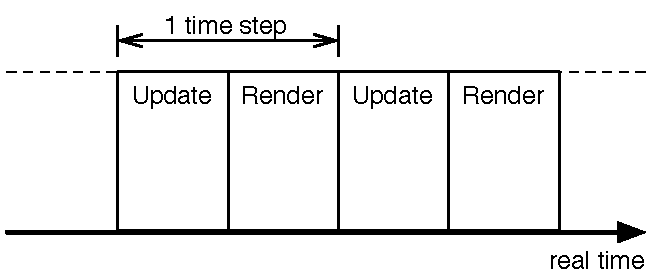
\includegraphics[scale = 0.8]{images/variableTimeStep} 
\caption{Variable time step.}
\label{fig:variableTimeStep}
\end{figure*}

With this simple approach, the FPS and UPS are variable. It is a problem because the physical simulation needs a fixed $\Delta t$ between two successive steps. At most, the difference should be little, which we cannot ensure with the previous design. Indeed, both the time to update the physical world and the one required to draw the objects on the screen are unpredictable due to the numerous factors that influence it. A thread can be preempt and thus slowed by the system, the number of objects do update and draw can change and, more specifically to our project, the number of rules to evaluate is variable. From the point of view of the user, the game could have different speeds on two devices and even during the simulation.

In order to have a fixed UPS, we introduce a sleeping period to synchronize all time steps. Figure \ref{fig:fixedTimeStep} shows the result when we have effectively the time to sleep after both \texttt{update} and \texttt{render}. The thread that runs the game loop, updating and drawing the game, is depicted on the top part of the time line. The android thread which handle all events as user inputs is on the bottom. We observe that all asynchronous events are stored during an entire time step (including the sleep) and then shared with the game engine at the beginning of the next step.

\begin{figure*}[h]
\centering
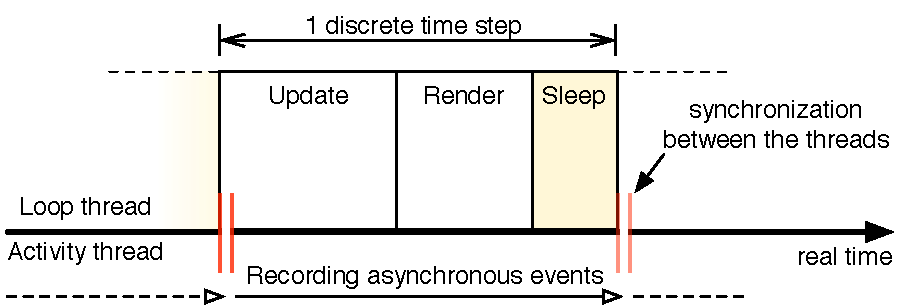
\includegraphics[scale = 0.8]{images/fixedTimeStep} 
\caption{Fixed time step.}
\label{fig:fixedTimeStep}
\end{figure*}


// EXPLAIN the missed frame


\begin{figure*}[h]
\centering
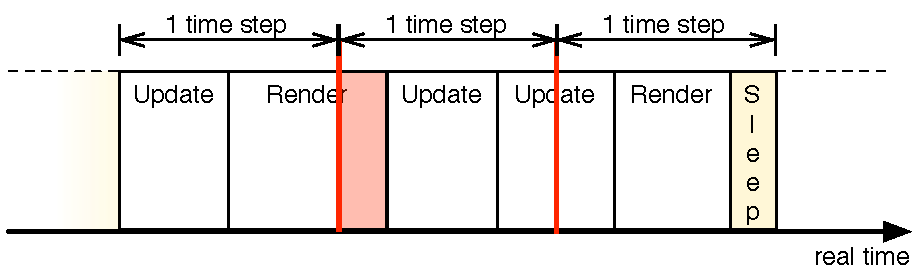
\includegraphics[scale = 0.8]{images/missFrame} 
\caption{Fixed time step with a missed frame.}
\label{fig:missFrame}
\end{figure*}

\section{Future work}


\section{Conclusion}



\end{document}